\documentclass{report}

\usepackage[utf8]{inputenc}
\usepackage[T1]{fontenc}
\usepackage[francais]{babel}
\usepackage{hyperref} % Pour les liens
% \usepackage{titlesec}
% \usepackage{microtype}
% \usepackage{blindtext}
\usepackage{graphicx}
\graphicspath{{images/}}
\newcommand{\hsp}{\hspace{15pt}}
% \titleformat{\chapter}[hang]{\Huge}{\thechapter{.}\hsp}{0pt}{\Huge}

\title{
    \begin{minipage}\linewidth
        \centering{
            RAPPORT DE PROJET \break
            "Cloud et virtualisation avec Openstack"
        }
    \end{minipage}
}
\author{
    \begin{minipage}\linewidth
        \centering{Tutrice : BOUZIANE Hinde\break}
        \break
        \centering{
            Groupe : \break
            CULTY Alexandre,\break
            BENAIS Charles,\break
            BRESSAND Jérémy,\break
            ROGLIANO Théo
        }
        \break
    \end{minipage}
}
\date{2016}

\begin{document}

\maketitle % Page de garde

\large % Pour la taille de la police

% ------------------------------ REMERCIEMENTS ------------------------------
\newpage
\chapter*{Remerciements}
    Nous tenons tout d'abord à remercier madame BOUZIANE Hinde, notre tutrice de projet, qui nous a permis de réaliser ce projet.\break

    Nous voulons aussi remercier l'équipe de Grid5000 qui nous à permis de réaliser ce projet sur leur système en nous donnant accès à leurs serveurs.



% ------------------------------ INTRODUCTION ------------------------------
\newpage
\chapter*{Introduction}
    \begin{quote}
        «Le cloud computing c'est l'exploitation de la puissance de calcul ou de stockage de serveurs informatiques distants par l'intermédiaire d'un réseau.» [Wikipédia]
    \end{quote}
    \bigbreak

    Dans les années 1950, les utilisateurs accédaient depuis leurs terminaux à leurs applications sur des serveurs appelés «mainframes», l'ancêtre du cloud computing.\break
    Dans les années 2000, les ASP (fournisseur de service d'application), apparaissent et hébergent des serveurs web, mails, etc.\break
    Le cloud est né à la suite de la multiplication des centres de données, de l'expension de la vitesse des communications et de la vitesse des calculs ainsi que de la maitrise de la virtualisation.\break

    L'intérêt du cloud tiens dans le fait que les serveurs sont loués à la demande, et que la facturation soit fait à l'usage. Autrement dit, le client paye uniquement l'utilisation réelle qu'il en a fait, pour les caractéristiques précises qu'il peut modifier.\break
    
    On distingue trois grands services de cloud :
    \begin{itemize}
        \item IaaS : Infrastructure as a Service, qui donne accès à des machines virtuelles sur lesquelles l'utilisateur peut installer son propre système d'exploitation et faire évoluer les caractéristiques du serveur à la demande (exemple : location d'un VPS).
        \item PaaS : Platform as a Service, l'utilisateur installe ses propres applications (exemple : installation de LAMP).
        \item SaaS : Software as a Service, les applications sont directement mis à disposition des utilisateurs, celui-ci ne s'occupe en rien de la gestion du serveur (exemple : utilisation d'un logiciel de VoIP).
    \end{itemize}
    \bigbreak
    
    Il existe aussi d'autres services, comme par exemple le DaaS (Data as a service), STaaS (Storage as a service), etc, mais les trois cités plus haut sont les plus populaires.\break
    
    En résumé, avec le cloud computing plus besoin de serveurs locaux à entretenir, tous les services sont accessible via internet et sont interconnectés.\break
    
    \begin{figure}
        \includegraphics[width=\textwidth]{responsabilites}
        \caption{Les responsabilités par service du cloud [Wikipédia]}
    \end{figure}


% ------------------------------ CONTENU ------------------------------
% --------------- 1 ---------------
\newpage
\chapter{OpenStack}
    \begin{figure}
        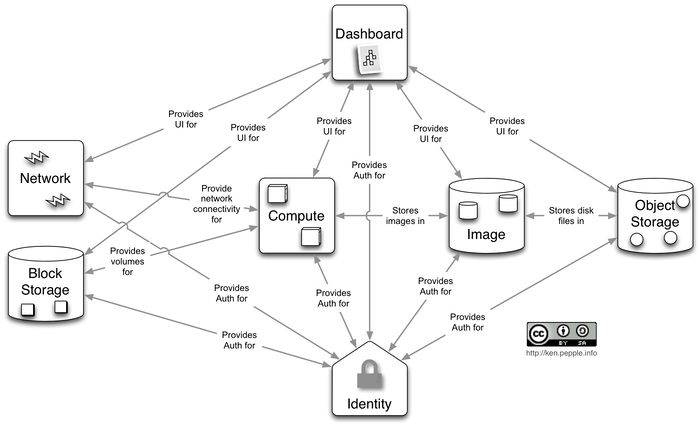
\includegraphics[width=\textwidth]{openstack_arch}
        \caption{Les responsabilités par service du cloud [Wikipédia]}
    \end{figure}

% --------------- 2 ---------------
\newpage
\chapter{Travail réalisé}
    \begin{quote}
        « The world will be distributed » Mark Collier, OpenStack Foundation
    \end{quote}
    \bigbreak
    \section{Mise en place}
        \subsection{Single machine}
            Dans le but de nous familiariser avec ce nouveau domaine,
            et l'accès à des machines possédant les droits administrateurs (sudo)
            ne nous étant pas offert à la faculté des sciences,
            nous avons choisi de mettre en place OpenStack sur nos machines personnelles.\break
            Devstack est un script bash automatisant la mise en place des modules OpenStack, 
            avec une configuration minimale.\break

        \subsection{Multi-nodes}
            Dans un second temps il nous à été offert l'opportunité de travailler sur les clusters
            de Grid5000, un Réseau de Ressources distribuées supporté par l'INRIA et le CNRS.\break
            Cela nous à permis de mettre en place un environnement de Cloud OpenStack stable et itérable, 
			dans le but d'offrir des démonstrations ou scénario de déploiement de machines virtuelles,
			utilisées comme support à une application, un programme ou plus simplement d'exemple de 
			configuration. (réseau)\break
			\subsubsection{Client-Serveur Chat}
			    Réseau de VM fermé
			\subsubsection{FTP}
				Réseau de VM ouvert sur conditions
			\subsubsection{Apache}
				Réseau de VM wide open

% --------------- 3 ---------------
\chapter{Problèmes rencontrés}
    \section{DevStack}
        Les premières semaines du TER, nous avons commencer par travailler OpenStack en utilisant DevStack, 
        qui permet d'installer différents modules de base OpenStack sur une unique machine.\break
        \subsection{Installation \& Configuration}
            DevStack requiert une configuration minimale, ainsi que des prérequis de configuration (systeme, 
            network).\break
            Il n'à pas été aisé de mettre en place cette configuration, et, quand bien même une configuration 
            DevStack ait été correctement mise en place et fonctionnelle, celle-ci n'à pour durée de vie qu'une session ! 
            
            
    \section{OpenStack sur Grid5000}
        Chacun rencontrant des difficultés lors du déploiement DevStack Mme. BOUZIANE à pu obtenir un accès au reseau 
        de Grid5000 afin de pouvoir utiliser les scénarios de déploiement d'OpenStack existants.\break
        \subsection{XP5K-OpenStack}
            



% ------------------------------ CONCLUSION ------------------------------
\newpage
\chapter*{Conclusion}


% ------------------------------ RESSOURCES DOCUMENTAIRES ------------------------------
\newpage
\chapter*{Ressources documentaires}
\href{http://docs.openstack.org/developer/devstack/}{Devstack} :
\url{http://docs.openstack.org/developer/devstack/}
\bigbreak
\href{http://www.openstack.org/}{Openstack} :
\url{http://www.openstack.org/}
\bigbreak
\href{https://www.grid5000.fr/}{Grid5000} :
\url{https://www.grid5000.fr/}
\bigbreak
\href{https://fr.wikipedia.org/wiki/Cloud_computing/}{Wikipédia} :
\url{https://fr.wikipedia.org/wiki/Cloud_computing/}



% ------------------------------ ANNEXES ------------------------------
\newpage
\chapter*{Annexes}



\end{document}

% --------------------------- INSTALLATION LATEX ----------------------
%sudo apt-get install texlive
%sudo apt-get install texlive-lang-french
%sudo apt-get install texlive-latex-extra
% Compile Time : pdflatex Rapport.tex
% Pensez à virer les .log, .aux, .out ET .pdf avant de push !
